\documentclass{article}
\usepackage{tikz}
\usepackage{amsmath}

\begin{document}

(28th February)
\section*{Combinatorics}
There are six lectures that need to be well understood for a test that comes in less than 2 weeks (\%20) QUIZ.

\begin{itemize}
				\item Permutations (Today)
				\item Subsets
				\item Set Partitions
				\item Integer Partitions
				\item Product Spaces (Gray Codes)
				\item Grade Coach
\end{itemize}

\section*{Permutations}
"Johnson Trotter" permutation enumeration algorithm...notation we speak of $[1, 2, ..., n] = [n]$.

Proposition: The number of permutations of $n$ objects of length $k$ is

\begin{equation}
				n(n-1)(n-2)...(n-k+1) = (n)_k
\end{equation}

Of course where the total number of permutations is $n!$...
And in combinatorics we want to do three things efficiently

\begin{itemize}
				\item Enumerate every permutation (each step constant amortized time, "fast")
				\item Map combinatorial object to an integer (ranking).
				\item Map a rank to re-build a combinatorial object (de-ranking).
\end{itemize}

\subsection*{Lexicographic Ordering}
We do the natural enumeration, but each step is not exactly constant, lots of shifting needs to occur hence we lean onto the "Johnson Trotter" style permutation enumeration approach.

\subsection*{Johnson Trotter}
Intuition really is like; {\em notice the swapping of the 3 simply "zigzagging"...}.

% must look at rendered view of this tree, ordering here is reversed due to growth=right...
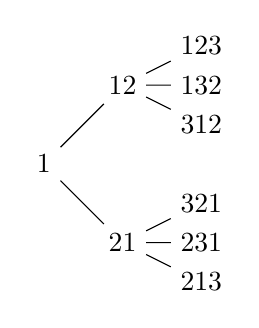
\begin{tikzpicture}[level distance=1cm,
  level 1/.style={sibling distance=2cm},
  level 2/.style={sibling distance=0.5cm},
	grow=right]
  \node {1}
    child {node {21}
      child {node {213}}
      child {node {231}}
      child {node {321}}
    }
    child {node {12}
      child {node {312}}
      child {node {132}}
      child {node {123}}
		};
\end{tikzpicture}

\subsection*{Ranking}
Recursive "stripping" definition; $n$ is the $n$th item of the list. $j$ is insertion position of the stripped $n$ in $\pi$.
  \[
    Rank(\pi) = n \cdot Rank(\pi_j) +
		\left\{\begin{array}{lr}
										j-1, & \text{if } Rank(\pi_j) \text{ is odd}\\
										n-j, & \text{if } Rank(\pi_j) \text{ is even}
        \end{array} \right\}
  \]

\subsubsection*{Example; Rank(31254)}
We construct down first like so; we stop when we try to compute a Rank of an ordered list. (as Rank is 0 in this case).
\begin{align}
				Rank(31254) &= 5 \cdot Rank(3124) + \text{ something}, j=4 \\
				Rank(3124) &= 4 \cdot Rank(312) + \text{ something}, j=4 \\
				Rank(312) &= 3 \cdot Rank(12) + \text{ something}, j=1
\end{align}

Now we build back up and populate all those "somethings", from the bottom using the ranking equation given...

\begin{align}
				Rank(31254) &= 5 \cdot Rank(3124) + (5 - 4) = (5 \cdot 8) + 1 = 41, j=4 \\
				Rank(3124) &= 4 \cdot Rank(312) + (4 - 4) = (4 \cdot 2) + 0 = 8, j=4 \\
				Rank(312) &= 3 \cdot Rank(12) + (3 - 1) = 0 + 2 = 2, j=1
\end{align}

\subsubsection*{Example; Rank(25134)}
Just repeating
\begin{align}
				Rank(25134) &= 5 \cdot Rank(2134) + \text{ something}, j=2 \\
				Rank(2134) &= 4 \cdot Rank(213) + \text{ something}, j=4 \\
				Rank(213) &= 3 \cdot Rank(21) + \text{ something}, j=3 \\
				Rank(21) &= 2 \cdot Rank(1) + \text{ something}, j=1
\end{align}

\begin{align}
				Rank(25134) &= 5 \cdot Rank(2134) + (2 - 1) = (5 \cdot 23 + 1) = 116, j=2 \\
				Rank(2134) &= 4 \cdot Rank(213) + (4 - 1) = (4 \cdot 5) + 3 = 23, j=4 \\
				Rank(213) &= 3 \cdot Rank(21) + (3 - 1) = (3 \cdot 1) + 2 = 5, j=3 \\
				Rank(21) &= 2 \cdot Rank(1) + (2 - 1) = 0 + 1 = 1, j=1
\end{align}

\subsection*{Un-ranking is omitted, we must read the books}

\end{document}
